\documentclass[12pt]{article}
\usepackage[utf8]{inputenc}
%\usepackage[T1]{fontenc}
%\usepackage{dejavu}
\usepackage{enumitem}

\usepackage{listings}
\usepackage{amsfonts}
\usepackage{fancyhdr}
\usepackage{comment}
\usepackage{graphicx}
\usepackage[letterpaper, top=2.5cm, bottom=2.5cm, left=2.2cm, right=2.2cm]{geometry}
%\renewcommand{\item}[1]{\item \textbf{#1}}
\begin{document}

\begin{center}
%\includegraphics{logo_unah.png}\\
\bfseries{Universidad Nacional Autónoma de Honduras}\\
Facultad de Ingeniería\\
Departamento de Ingeniería en Sistemas\\
\bigskip
\bigskip
Asignatura: IS-611 Redes de Datos 2\\
Impartida  por José Mario López
\end{center}
\begin{center}
\noindent\rule{\textwidth}{1pt}
\huge{Práctica de Integración de protocolos de enrutamiento dinámico}\\
\vspace{10px}
\small{Redistribución de rutas entre origenes de enrutamiento}
\noindent\rule{\textwidth}{1pt}
\end{center}

%\title{Resumen sobre Spanning-Tree Protocol}
 %\author{José Mario López}
 %\date{\today}
%\maketitle
\section{Introducción} 
El objetivo de esta práctica es adquirir y reforzar habilidades en configuración de protocolos de enrutamiento dinámico: EIGRP, y OSPF de una sola área; comprender su funcionamiento y la redistribución de rutas entre diferentes orígenes de enrutamiento.

\section{Topología}
Se presenta una topología conformada por dos zonas. Cada zona debe ser configurada con el un protocolo de enrutamiento dinámico, como indica la siguiente figura (los nombres de la figura son ilustrativos, luego se pide que usted los cambie):

\begin{figure}[h]
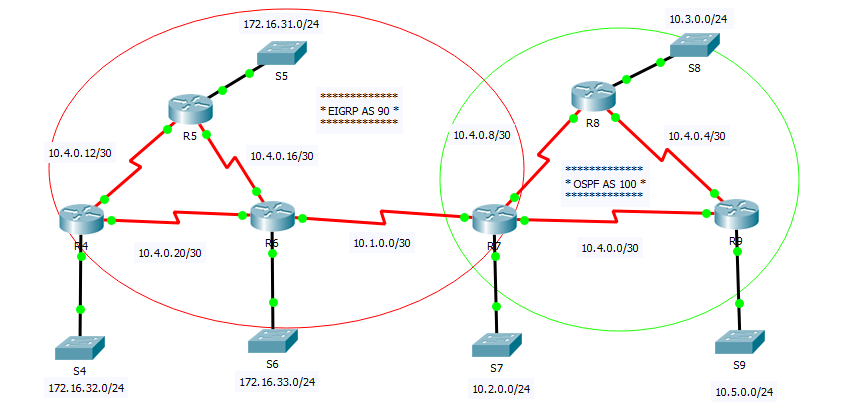
\includegraphics[scale=0.9]{img_pr4.PNG}
\end{figure}

\begin{itemize}
\item Para el Área B utilice EIGRP, con sistema autónomo 90.
\item Para el Área C utilice OSPF, con sistema autónomo 100 y área 0.
\end{itemize}

\section{Actividades Obligatorias (valor: 60\%)}
\subsection{Crear la topología utilizando Packet Tracer}
\begin{enumerate}[label=\Alph*]
\item Utilice routers modelo 2811, y añada módulos WIC-2T para contar con interfaces seriales.
\item Utilice switches modelo 2960, de 24 puertos.
\end{enumerate}

\subsection{Configuraciones básicas}
\begin{enumerate}[label=\Alph*]
\item Cambie el hostname en los routers. Asigne la letra R, con el número que corresponda, seguido del protocolo que ejecuta. e.g. R4EIGRP, o R7EIGRP-OSPF (separe con un guión los nombres de los procotolos, si ejecuta más de uno.)
\item \textit{\textbf{Configure logging synchronous para evitar que los mensajes en consola, interfieran con la escritura de comandos}}
\end{enumerate}

\subsection{Configurar el direccionamiento IPv4 de cada zona}


\begin{enumerate}[label=\Alph*]
\item Configurar los gateway utilizando la primera dirección utilizable del bloque de direccionamiento disponible para cada red.
\item Configurar las direcciones IP de las interfaces seriales, de los enlaces entre routers. Utilice un clock rate de 64000.
\item Añada un host a cada switch, cuando sea necesario, para realizar las pruebas de conectividad requeridas.
\end{enumerate}

\textit{\textbf{Asegúrese de guardar las configuraciones en cada router, y guardar el archivo de packet tracer.}}

\subsection{Configurar los protocolos de enrutamiento}
Después de cada configuración, haga las pruebas de conectividad correspondientes.
Configure no auto-summary en el protocolo correspondiente.

¿Cuál es la utilidad de desactivar el resumen automático de rutas?

\begin{enumerate}[label=\Alph*]
\item Configure EIGRP en la zona B, utilice el comando network seguido de la dirección de red que va a anuciar, y la wildcard respectiva. Asegúrese que todos los routers tiene rutas para llegar a las subredes de la misma zona.
\item Verifique las tablas de enrutamiento de cada router para comprobar que tienen las rutas para cada red local.

\item Configure OSPF en la zona C. Utilice el comando network con la dirección de red respectiva y la wildcard.

Asegúrese que todos los routers tiene rutas para llegar a las subredes de la zona. 
\item En R7 configure EIGRP y OSPF. \textit{En EIGRP solo agregue la red 10.1.0.0/30}

En este punto, el R7 debe tener en su tabla de enrutamiento las rutas aprendidas con EIGRP y con OSPF.
\end{enumerate}

\textit{\textbf{Asegúrese de guardar las configuraciones en cada router, y guardar el archivo de packet tracer.}}

\subsection{Redistribución de información de enrutamiento}
Como podrá observar en el router R7, En un mismo equipo pueden estar funcionando varios procesos de procotolos de enrutamiento, pero no intercambian información entre ellos. 

Para obtener una red convergente en una topología multiprotocolo, se hace necesario configurar cuestiones adicionales:

\subsubsection{Redistribución de rutas en OSPF}

\textbf{Redistribuir  rutas de EIGRP dentro del proceso OSPF.}

\begin{lstlisting}
Router(config-router)#redistribute eigrp [AS] subnets 
\end{lstlisting}
\vspace{10px}
\textbf{Redistribuir rutas de RIP dentro del proceso OSPF.}
\begin{lstlisting}
Router(config-router)#redistribute rip subnets
\end{lstlisting}

\subsubsection{Redistribución de rutas en EIGRP}
Los valores que se indican después del parámetro \textit{metric} los utiliza DUAL para calcular la métrica.

\textbf{Redistribuir  rutas de RIP dentro del proceso EIGRP}
\begin{lstlisting}
Router(config-router)#redistribute rip metric 10000 10 255 1 1500
\end{lstlisting}
\vspace{10px}
\textbf{Redistribuir  rutas de OSPF dentro del proceso EIGRP.}
\begin{lstlisting}
Router(config-router)#redistribute ospf [ID] metric 10000 100 255 1 1500
\end{lstlisting}

\subsubsection{Redistribución de rutas en RIP}
\textbf{Redistribuir  rutas de EIGRP dentro del proceso RIP}
\begin{lstlisting}
 Router(config-router)#redistribute eigrp [AS] metric 2
\end{lstlisting}
\vspace{10px}
\textbf{Redistribuir  rutas de OSPF dentro del proceso RIP.}
\begin{lstlisting}
Router(config-router)#redistribute ospf [ID] metric 2
\end{lstlisting}
\vspace{15px}
%%%%%%%%%%%%%%%%%%%%%%%%%%
\subsection{Actividades complementarias (valor: 40\%) }
\subsubsection{Redistribución de rutas}
\begin{enumerate}[label=\Alph*]
\item En R7, redistribuya las rutas de OSPF dentro de EIGRP. Verifique las tablas de enrutamiento. ¿Cuál es el código asignado a las rutas externas a EIGRP? \_\_\_\_\_\_\_\_\_\\
¿Cuál es la métrica para las rutas redistribuidas de esta manera? \_\_\_\_\_\_\_\_\_

\item En R7, redistribuya las rutas de EIGRP dentro de OSPF. Verifique las tablas de enrutamiento.
¿Cuál es el código asignado a las rutas redistribuidas de esta manera? \_\_\_\_\_\_\_\_\_\\
¿Cuál es la métrica para las rutas externas a OSPF? \_\_\_\_\_\_\_\_\_\\

En este punto debe haber conectividad entre todos los host, si no es así, realice el proceso de resolución problemas. \_\_\_\_\_

\item En R7, redistribuya las rutas de OSPF dentro de EIGRP. Siga el comando tal como se muestra en el apartado 3.5.2 Es probable que no haya una redistribución. Después se abordará ese inconveniente, puede proseguir con su práctica.
\end{enumerate}
\subsubsection{Configuración de comandos básicos}
\begin{enumerate}
\item Configure los hostname de los routers de la topología. R + número de router + protocolo que ejecuta. Si ejecuta dos, sepárelos con un guión ( - )
\item Configure las contraseñas de acceso por consola en todos los routers de la zona A, y logging synchronous.
\item Configure las contraseñas de acceso por telnet (lineas VTY), y contraseña enable en los routers de la zona B. 
\item Configure el comando Banner motd con un mensaje de advertencia de acceso no autorizado, en los routers de la zona C.
\item Configure el servicio DHCP en cada router para la asignación dinámica de direccionamiento.
\item Complete la configuración (en los routers) de todos los comandos básicos.
\end{enumerate}

\vfill

\vfill
{\textbf {\normalsize José Mario López}}

{\small Profesor de la asignatura\\}

{\footnotesize 
De presentarse alguna duda respecto al contenido del documento, recuerde que puede abocarse al Departamento de Ing. En Sistemas, en hora de consulta, de lunes a viernes; o enviar un correo a jmlopezc@unah.edu.hn}
\end{document}